\chapter{Vulnerability Notification Tool}
\label{chap5-vulnerability-notification-tool}
\thispagestyle{empty}

\section{Motivation}

\paragraph{}
Every day new vulnerabilities and security updates are announced. Some of these vulnerabilities affect CERN websites or web servers and could be critical. Therefore, it is important to learn about them as soon as possible and notify the owners of the affected resources to take necessary actions, i.e., patch or update their resource. The current procedure in CERN security team for managing vulnerabilities is as follows:
\begin{enumerate}
\item Getting informed about vulnerabilities from various sources by monitoring public databases, project mailing lists, security mailing lists, twitter accounts, blogs, etc.
\item Deciding if a vulnerability is worth investigating and is likely to affect CERN (human decision)
\item In case of vulnerabilities related to web applications, the next step is to review the output of WAD on all CERN websites and web servers, in order to get a list of resources that could be affected.
\item Sending notifications to the resource owners after making sure that the resource is in fact vulnerable, i.e., runs the vulnerable version or has a vulnerable configuration.
\end{enumerate}

The main goal of the Vulnerability Notification Tool(VNT) is to automate this procedure as much as possible and optimize each step of the process.Staying up-to-date with vulnerability sources and announcements is a time consuming task and we still do not know if we are monitoring the best sources. With the current procedure we might ignore some vulnerabilities that are important for CERN, but do not create much noise in the public. 
On the other hand, there are so many vulnerabilities that are published every day, so even if we get informed about all vulnerabilities, it is impossible to investigate every single one of them. 

Figure \ref{figure:vulns_per_year}
\footnote{Picture taken from \url{http://web.nvd.nist.gov/view/vuln/statistics-results?adv_search=true&cves=on&pub_date_start_month=0&pub_date_start_year=2000&pub_date_end_month=11&pub_date_end_year=2014}} shows the trend in the number of vulnerabilities published in the last 15 years. Apparently, 2014 with almost 8000 vulnerabilities has been the worst year for security. Due to the ever increasing volume of public vulnerability reports, CVE MITRE has even updated the CVE-ID syntax since January 2015. The new syntax, unlike the previous 4 digit one, allows to identify more than 9999 vulnerabilities each year.\footnote{\url {https://cve.mitre.org/cve/identifiers/syntaxchange.html}}. 
\\
The Vulnerability Notification Tool(VNT) tries to save the organization time by filtering out the non-critical vulnerabilities or the vulnerabilities that do not affect CERN, so that more time can be spent on remediation rather than detection of the vulnerabilities.


\begin{figure}[h!]
\label{figure:vulns_per_year}
  \centering
    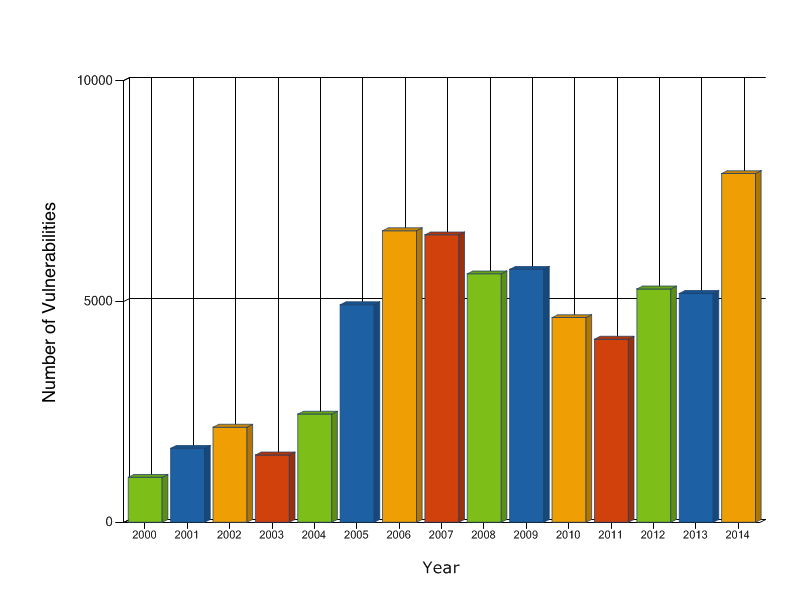
\includegraphics[width=1.0\textwidth]{vulns_per_year}
  \caption{Number of Vulnerabilities Per Year}
  
\end{figure}

%\section{Related Work}
%
%\subsection{Cassandra}

\section{Source Evaluation}
\paragraph{}
There are plenty of public sources that announce vulnerabilities or maintain a database of all vulnerabilities over years. The performance of the Vulnerability Notification Tool very much depends on the quality of the source it is using. Obviously, it is not possible to find a perfect source. For example, there is a trade-off between the speed of publishing the vulnerabilities and accuracy of the information published; hence, it is crucial to know the needs of the organization and choose the best fitting source.

\subsection{Approach}
\paragraph{}
In order the evaluate the vulnerability sources the following evaluation factors have been considered:
\begin{enumerate}
\item \textbf{Completeness}: Does the source contain all the vulnerabilities that CERN would probably care about? 
\item \textbf{Speed}: How long since the disclosure does it take for the vulnerability to be published?
\item \textbf{Information Quality}: What information( e.g., severity level, exploits, solutions) about a vulnerability is published?
\item \textbf{Parsable Feed} Does the source provide a parable feed that can be downloaded and updated automatically?
\end{enumerate} 

Table \ref{table:sample_vulns} contains 6 vulnerabilities published over the last few months. These vulnerabilities have been used as case studies to evaluate completeness and speed of different sources. These vulnerabilities were of great importance for CERN and can be a good indicator of how well a source fits CERN needs.
\begin{table}
\begin{center}
    \begin{tabular}{ | c | c | c| }
    
    \hline
    \hhline{|*3-}
	\rowcolor{LightBlue}    
    \textbf{Vulnerability} & \textbf{CVE-ID} & \textbf{Disclosure Date} 
    %& Summary 
    \\ \hline
    GitLab groups API & CVE-2014-8540 & 30.10.2015
%     & The vulnerability allows a guest user to delete the owner of a group and to assign any other member as owner through the groups API.
      \\ \hline
    Wordpress 4.0.1 Security Release & CVE-2014-9032(*)  & 20.11.2014
    % & XSS vulnerability allows remote attackers to inject arbitrary web script or HTML via unspecified vectors.[...]\footnote{\url{https://wordpress.org/news/2014/11/wordpress-4-0-1/}} 
    \\ \hline
    Drupal SQL injection
 & CVE-2014-3704
 & 15.10.2014 
 %& The vulnerability allows remote attackers to conduct SQL injection attacks via an array containing crafted keys
  \\
    \hline

 Poodle
 & CVE-2014-3566
 & 14.10.2014
 %& The SSL protocol 3.0 allows man-in-the-middle attackers to obtain clear text data via a padding-oracle attack
  \\
    \hline

Twiki Remote Code Execution
 & CVE-2014-7236
 & 09.10.2014
 %& The debugenableplugins request parameter allows arbitrary Perl code execution.  
 \\
    \hline

ShellShock
 & CVE-2014-6271
 & 24.09.2014
 %& Via certain applications, a local or remote attacker may inject shell commands, allowing local privilege escalation or remote command execution depending on the application vector. 
  \\
    \hline

    \end{tabular}
    \caption{Sample vulnerabilities}
    \label{table:sample_vulns}
     \footnotesize{(*) This update fixes multiple vulnerabilities (CVE-2014-9032,CVE-2014-9033,CVE-2014-9034,CVE-2014-9035,CVE-2014-9036,CVE-2014-9037)}
   \end{center}
   
\end{table}


\subsection{Vulnerability Sources}

\paragraph{}
There are plenty of mailing lists, databases, vulnerability sources,etc., available online and each of these sources provide different types of information for different purposes. A part of this project was to do some research on these different sources and compare them with respect to CERN needs. In this section, we will give a summary of the sources that were evaluated. 
\begin{itemize}
\item \textbf{Natinal Vulnerability Database (NVD)}\footnote{\url{https://nvd.nist.gov/}}: The U.S. government repository of standards based vulnerability management data
\item \textbf{Open Sourced Vulnerability Database (OSVDB)}\footnote{\url{www.osvdb.or}}: An independent and open sourced\footnote{The data is collected from publicly available sources} web-based vulnerability database created for the security community. 
\item \textbf{CVE Details}\footnote{\url{http://www.cvedetails.com/}}: Provides CVE vulnerability data and statistics about vendors and products through a web interface
\item \textbf{Secunia Vulnerability Intelligence Manager (VIM)}\footnote{\url{http://secunia.com/vulnerability_intelligence}}: Provides a filtered feed of verified vulnerability intelligence in real-time.

\end{itemize}

Table \ref{table:source_speed} illustrates the publication date of sample vulnerabilities on individual sources. If a source is missing a particular vulnerability the corresponding cell is going to be empty. Using this table we can compare the completeness and speed of different sources. Note that in each row, the fastest source is marked in green, the slowest in red and the average ones in yellow. Taking a glance at the table, we realize that OSVDB has the highest publication speed and is the most complete source.
\\
The comparison of the information quality and data feeds is illustrated in table \ref{table:source_evaluation}. NVD provides free XML data feeds. OSVDB provides information via the web interface as a free resource for the community. Alternate methods of obtaining the data such as API or exports are no longer supported via OSVDB and are offered by Risk Based Security as a commercial product, called VulnDB API. CVE Details offers JSON feeds for the vulnerabilities, but unfortunately, the feeds are not complete and they do not contain vulnerable product information which is one of the most important fields for the purpose of VNT. Secunia VIM is also a commercial product\footnote{A trial account was used for evaluation} and it provides vulnerability information via a web portal. It is possible to download XML description of vulnerabilities limited to the last 72 hours; however, the main focus of VIM is on vulnerability management through the graphical web interface. 

\begin{table}
\begin{center}
    \begin{tabular}{ | c || c | c | c | c | c | c |}
    
    \hline
	
      Vulnerability(*) & \textbf{NVD}  &  \textbf{OSVDB} & \textbf{CVE Details} & \textbf{Secunia VIM} 
	\\ 
	\hline  
	\hhline{~|*4-}  
	\textbf{GitLab} & \multicolumn{1}{|c|}{\cellcolor{red!25}} & \multicolumn{1}{|c}{\cellcolor{green!25} 31.10.2014} & \multicolumn{1}{|c|}{\cellcolor{red!25}} & \multicolumn{1}{|c|}{\cellcolor{red!25}} 
    \\ 
	\hline   
	\hhline{~|*4-} 
	 \textbf{Wordpress} & \multicolumn{1}{|c|}{\cellcolor{yellow!25} 25.10.2014} & \multicolumn{1}{|c}{\cellcolor{green!25} 21.10.2014} & \multicolumn{1}{|c|}{\cellcolor{red!25}} & \multicolumn{1}{|c|}{\cellcolor{green!25} 21.10.2014} 
	  \\ 
	\hline
	\hhline{~|*4-} 
	 \textbf{Drupal} & \multicolumn{1}{|c|}{\cellcolor{yellow!25}17.10.2014} & \multicolumn{1}{|c}{\cellcolor{yellow!25}17.10.2014} & \multicolumn{1}{|c|}{\cellcolor{yellow!25}17.10.2014} & \multicolumn{1}{|c|}{\cellcolor{green!25}16.10.2014}
	  \\ 
	\hline
	\hhline{~|*4-} 
	 \textbf{Poodle} & \multicolumn{1}{|c|}{\cellcolor{yellow!25}16.10.2014} & \multicolumn{1}{|c}{\cellcolor{yellow!25}19.10.2014} & \multicolumn{1}{|c|}{\cellcolor{yellow!25}16.10.2014} & \multicolumn{1}{|c|}{\cellcolor{green!25}15.10.2014}
	  \\ 
	\hline 
	\hhline{~|*4-} 
	 \textbf{Twiki} & \multicolumn{1}{|c|}{\cellcolor{red!25}} & \multicolumn{1}{|c}{\cellcolor{green!25} 09.10.2014} & \multicolumn{1}{|c|}{\cellcolor{yellow!25} 11.10.2014} &\multicolumn{1}{|c|}{\cellcolor{red!25}}
	  \\ 
	\hline 
	\hhline{~|*4-} 
	 \textbf{ShellShock} & \multicolumn{1}{|c|}{\cellcolor{green!25}25.09.2014} & \multicolumn{1}{|c}{\cellcolor{green!25}25.09.2014} & \multicolumn{1}{|c|}{\cellcolor{green!25}25.09.2014} &\multicolumn{1}{|c|}{\cellcolor{green!25} 25.09.2014} 
	 \\
	 \hline
    %\hhline{|*5-}
     
%\hhline{~~|-|~|-|}
%Critical\textsuperscript{*} & 190  & \multicolumn{1}{|c||}{\cellcolor{green!25}9}  & 622  & \multicolumn{1}{|c|}    
\end{tabular}
    \caption{Vulnerability Publication Dates}
    \label{table:source_speed}
    \footnotesize{(*) For the complete name of the vulnerability refer to table \ref{table:sample_vulns}}
   \end{center}
    \end{table}




\begin{table}
\begin{center}
    \begin{tabular}{ | c || c | c | c | c | c | c |}
    
    \hline
	 
      Data & \textbf{NVD}  &  \textbf{OSVDB} & \textbf{CVE Details} & \textbf{Secunia VIM} 
	\\ 
	\hline  
	\hhline{~|*4-}  
	\textbf{Description} & \multicolumn{1}{|c|}{\cellcolor{green!25}\cmark} & \multicolumn{1}{|c|}{\cellcolor{green!25}\cmark}
	& \multicolumn{1}{|c|}{\cellcolor{green!25}\cmark}& \multicolumn{1}{|c|}{\cellcolor{green!25}\cmark}
    \\ 
	\hline   
	\hhline{~|*4-} 
	 \textbf{Severity} & \multicolumn{1}{|c|}{\cellcolor{green!25}\cmark} & \multicolumn{1}{|c|}{\cellcolor{green!25}\cmark}
	& \multicolumn{1}{|c|}{\cellcolor{green!25}\cmark}& \multicolumn{1}{|c|}{\cellcolor{green!25}\cmark}
	  \\ 
	\hline
	\hhline{~|*4-} 
	 \textbf{Product} & \multicolumn{1}{|c|}{\cellcolor{green!25}\cmark} & \multicolumn{1}{|c|}{\cellcolor{green!25}\cmark}
	& \multicolumn{1}{|c|}{\cellcolor{green!25}\cmark}& \multicolumn{1}{|c|}{\cellcolor{green!25}\cmark}
	  \\ 
	\hline
	\hhline{~|*4-} 
	 \textbf{Exploits} & \multicolumn{1}{|c|}{\cellcolor{red!25}\xmark} & \multicolumn{1}{|c|}{\cellcolor{red!25}\xmark}
	& \multicolumn{1}{|c|}{\cellcolor{green!25}\cmark}& \multicolumn{1}{|c|}{\cellcolor{red!25}\xmark}
	  \\ 
	\hline 
	\hhline{~|*4-} 
	 \textbf{Solution} & \multicolumn{1}{|c|}{\cellcolor{red!25}\xmark} & \multicolumn{1}{|c|}{\cellcolor{green!25}\cmark}
	& \multicolumn{1}{|c|}{\cellcolor{red!25}\xmark}& \multicolumn{1}{|c|}{\cellcolor{green!25}\cmark}
	  \\ 
	\hline 
	\hhline{~|*4-} 
	 \textbf{Vulnerability Type} & \multicolumn{1}{|c|}{\cellcolor{green!25}\cmark} & \multicolumn{1}{|c|}{\cellcolor{green!25}\cmark}
	& \multicolumn{1}{|c|}{\cellcolor{green!25}\cmark}& \multicolumn{1}{|c|}{\cellcolor{green!25}\cmark}
	 \\
	 \hline	 
\hhline{~|*4-} 
	 \textbf{Feed} & \multicolumn{1}{|c|}{\cellcolor{green!25}\cmark} & \multicolumn{1}{|c|}{\cellcolor{yellow!25}VulnDB}
	& \multicolumn{1}{|c|}{\cellcolor{yellow!25}\cmark}& \multicolumn{1}{|c|}{\cellcolor{yellow!25}\cmark}
	 \\
	 \hline
    %\hhline{|*5-}
     
%\hhline{~~|-|~|-|}
%Critical\textsuperscript{*} & 190  & \multicolumn{1}{|c||}{\cellcolor{green!25}9}  & 622  & \multicolumn{1}{|c|}    
\end{tabular}
    \caption{Source Evaluation (Data and Feed)}
    \label{table:source_evaluation}
   \end{center}
    \end{table}
     
\subsection{Conclusion}
Downloading the latest vulnerability information automatically is one of the requirements of the tool. In addition, the tool is supposed to analyze the vulnerability data to filter out the non-critical and non-related vulnerabilities; therefore, it is important that the vulnerability information is represented in a structured and parsable format. 
The only sources that provide a useful parsable feed are NVD, OSVDB and Secunia VIM. Secunia VIM focuses on vulnerability management, assuming that there is human using its portal and taking necessary actions. There is no easy way of connecting it to another tool, i.e. WAD, and it is missing an API access. Although an XML description of vulnerabilities from last 72 hours can be downloaded in a semi-automatic way, by using tools like wget, we decided not to go for Secunia VIM, because buying the whole product and using only a non-main functionality of it was not beneficial.
\\
Tables \ref{table:source_speed} and \ref{table:source_evaluation} show it clearly that OSVDB is faster, more complete and more informative than NVD. In spite of that, NVD was the source we finally used for implementation of the tool, because OSVDB is offering the API access and its feed commercially (under the name VulnDB API) and due to business reasons we were not able to acquire the license.
\\
Although it was not been a decision factor, it is worth mentioning that vulnerability databases use different methods of abstraction. Some, like CVE, keep one entry per vulnerability, while some others, like Secunia VIM, create multiple entries for the same vulnerability, because there are different patches available (on different operating systems, for example).

\section{National Vulnerability Database}
\paragraph{}
NVD is the U.S. government repository of standards based vulnerability management data and it contains 68054 CVE vulnerabilities. It is recommended by CVE MITRE\footnote{https://cve.mitre.org/} to obtain infomation about a vulnerability severity rating, fix information,vulnerable software versions, etc. 
 
\subsection{Data Feeds}
The entire NVD can be downloaded on its web page for free and for public use. The XML vulnerability feed contains security related software flaws. Each vulnerability in the file includes a description and associated reference links from the CVE dictionary feed, as well as a CVSS base score\footnote{Common Vulnerability Scoring System is a standard measurement system for rating the severity of IT vulnerabilities}, vulnerable product configuration, and weakness categorization. The feed provides vulnerability information since 1999 (one file for each year, except that the file from 2002 includes all vulnerabilities published in 2002 and before). In addition, there is a ``recent'' feed, listing recently published vulnerabilities and a ``modified" feed, which provides the list of recently published and modified vulnerabilities, where "recently" is defined as the previous eight days. The feeds are updated approximately every two hours.

\section{Specifications}
Vulnerability Notification Tool is a tool that downloads the latest "modified" feed from NVD, finds the vulnerabilities that are newly published or have been changed since its last execution and for each of these vulnerabilities reports CVE-ID, description, CVSS score, published date and time, last modified date and time, and a list of affected software (vulnerable softwares in CPE format). In addition, the tool lists the URL of the CERN websites and web servers that are likely to have this vulnerability.

\subsection{Challenges}
\subsubsection{Downloading}
NVD keeps no history of the changes, you might miss some changes
The "modified" feed from NVD contains the latest vulnerabilities published or modified in the last 8 days. Obviously, if the tool is not run for more than eight days, it will definitely miss some updates. This issue can be fixed by looking at the yearly feed and detecting if a vulnerability information has changed in that feed since the last execution. Anyhow, it was decided that the tool will be running at least once a day and therefore there is no need for consulting the yearly feeds. 
Another point worth mentioning is that NVD keeps no record of the changes that happen in vulnerability data. It is impossible to see how a vulnerability has changed over time, because new data is always overwriting the old one. Vulnerability Notification Tool does not care about any intermediate changes in a vulnerability information between two consequent execution, but for a complete evaluation of the tool and in order to be able to simulate the tool over a period of time, we kept a local copy of the "modified" from downloaded daily since October 31\textsuperscript{th}, 2014. 
\subsubsection{Modification Date}
As NVD provides the last modified date as one of the fields in vulnerability information, the easiest way to find the vulnerabilities that have changed since the last execution of the tool, would be to compare their last modified time with the time of the last execution. However we discovered that this will not work as the last modified time reported by NVD is not always 100 percent reliable. Imagine there is a vulnerability X published at time t$_{\text{0}}$. If we look at the NVD feed at time t$_{\text{2}}$ we see that the last modified time for the vulnerability is t$_{\text{0}}$, which means that the vulnerability has not changed since its publication. Now we look at the vulnerability at time t$_{\text{3}}$ and to our surprise we see that the last modified time is t$_{\text{0}}$<t$_{\text{1}}$<t$_{\text{2}}$. If we compare this time to the last execution time (t$_{\text{2}}$) we might decide to ignore the vulnerability and assume it has not changed, which is not correct. A script was written to check for existence of this case in NVD feeds and many instances of this controversy was found. For example on 05.11.2014 the last modified time of CVE-2012-5500 was reported as 03.11.2014 and if we check for the same vulnerability on 06.11.2014 we get the last modified time as 04.11.2014. In addition we observed that sometimes the details of a vulnerability, such as its CVSS score might change without changing the last modified field. Due to these problems we decided to ignore the last modified time field completely and came up with the following solution to find updated vulnerabilities. 
The general idea is to keep a local copy of vulnerability information (a JSON file per vulnerability). For each vulnerability in a new feed we look at our local version of that vulnerability. If there is no local version, the vulnerability is reported as newly published and its data is stored locally, otherwise we compare the local version with the new data, report the changes and overwrite the old data with the new one. 
This solution solves the modification time problem and makes it possible to report what exactly has changed in a vulnerability. 

\subsection{Vulnerable Configuration}
In addition to the list of vulnerable software, NVD provides a list of vulnerable configurations. For example if Safari 5.0.5 is vulnerable only on Mac OS X 10.5.8 the vulnerable software list would contain Safari 5.0.5 but no information about the operating system. In this case it would be useful to extract the configuration data from NVD and use it to make sure that a resource is vulnerable. Given the scope of this project, unavailability of configuration specifications on CERN resources and the fact that only a few vulnerabilities are bound to a specific configuration, we decided to ignore this field and only report the data from vulnerable software list field. 

\section{Product Name Matching}

The next step after extracting the new and modified vulnerabilities is to find the CERN resources that might be affected by these vulnerabilities. As an intermediate step it is important to find which WAD names are affected by each vulnerability. If we know about the affected WAD names, finding the resources is an easy task of going over WAD output on all websites and web servers at CERN and reporting the URLs. 
\subsection{Common Platform Enumerations}
The Common Platform Enumeration (CPE) is a structured naming schema for IT systems, platforms and packages. It aims at providing a formal, consistent and uniform naming schema, so that the community members are able to generate names for new IT platforms in a consistent and predictable way \ref{fsdfdF}. This will facilitate automation in security practices. CPE is based on the generic syntax for Uniform Resource Identifiers and each name consists of the prefix "cpe:" and specifies either a hardware (h), operating system (o), or application environment (a). Each element consists of one or more components, separated by colons. The first component names the vendor or supplier of the element; subsequent components provide additional information. \ref{dfsdf} 
Table ???? contains some examples of CPE. 

\begin{table}
\begin{center}
    \begin{tabular}{ | c | c | }
    
    \hline
	 
    CPE & Description  
    \\ \hline
    % cpe:/o:microsoft:windows_xp:::home
    % cpe:/h:samsung:galaxy_note_2:-"
    % cpe:/a:wordpress:wordpress:1.0
    \multirow{3}{*}{\texttt{cpe:/h:samsung:galaxy\_note\_2:-}} & Samsung Galaxy Note 2 \\ & (Hardware) \\ & 
        \\ \hline
   \multirow{3}{*}{\texttt{cpe:/o:microsoft:windows\_xp:home}} & Microsoft Windows XP \\ & Home Edition \\ & Operating System
        \\ \hline
         \multirow{3}{*}{\texttt{cpe:/a:wordpress:wordpress:1.0}} &  \\ & Wordpress 1.0 \\ & 
        \\ \hline
    \end{tabular}
    \caption{CPE Examples}
    \label{table:sample_cpes}
   \end{center}
    
\end{table}

In this project we only care about vulnerabilities that affect operating systems or applications and we can ignore the hardware related vulnerabilities when mapping CPE to WAD names. As you can see in the examples, the first three components of the CPE (after the type indicator) are the ones that describe the vulnerable in the format of \framebox[1.0\width]{\texttt{\{vendor\}:\{name\}:\{version\}}}.
 

\subsection{WAD Product Names}

As already discribed in section ????? 1.3.3 WAD uses the detection rules coming from Wappalyzer[???] and Wappalyzer is an open source browser plugin with a community of over 100 contributors. Wappalyzer is using no standard in naming the technologies it detects and it mostly relies on the contributor's common sense to choose a meaningful name for each technology. As of the time of writing this thesis Wappalyzer detects 707 technologies{\footnote{\texttt{cert was wad\_list -apps | wc -l}} from 50 different categories{\footnote{\texttt{cert was wad\_list -categories | wc -l}}. 
\subsubsection{Challenges}
The lack of using a standard naming approach in Wappalyzer and consequently in WAD, makes it difficult to match CPE names to WAD names. On the other hand, CPE itself is not 100\% consistent and sometimes for the same application one can find multiple CPE names, as an example \texttt{cpe:/a:django\_piston\_project:django\_piston:0.2.2.0} \texttt{cpe:/a:djangoproject:django\_piston:0.2.2.0} and \texttt{cpe:/a:djangoproject:piston:0.2.2.0} are valid CPE names that have been seen in NVD XML feeds, but they all refer to the same application.
There is an official CPE dictionary available online that is supposed to provide an agreed upon list of official CPE names[???]. Unfortunately we noticed that many of the CPE names that appear on NVD vulnerability feeds are not present in this dictionary and therefore there is no way of knowing which CPEs we are going to find in vulnerability feeds in advance. Considering the CPE dictionary as well as all the vulnerabilities published on NVD websites, currently there are 33615 number of unique CPE names (considering the vendor and product name and ignoring other components such as version)\footnote{Look at appendix ???? for the methode}. Table \ref{table:cpe_wad_mapping} tries to show how irregular the namings are. As you can see sometimes the vendor name appears in the WAD name and sometimes not. Or the word separator can be a space character, a period, an underscore, etc. 

\begin{table}
\begin{center}
    \begin{tabular}{ | c | c | }
    
    \hline
	 
    CPE & WAD Name  
    \\ \hline
    % cpe:/o:microsoft:windows_xp:::home
    % cpe:/h:samsung:galaxy_note_2:-"
    % cpe:/a:wordpress:wordpress:1.0
    \texttt{cpe:/a:adobe:coldfusion:8.0} & Adobe ColdFusion 
        \\ \hline
    \texttt{cpe:/a:yandex.metrics\_project:yandex\_metrics:1.0} & Yandex.Metrika
        \\ \hline
    \texttt{cpe:/a:woothemes:woocommerce\_plugin:2.1.0} & WooCommerce
        \\ \hline
 	\texttt{cpe:/a:djangoproject:django:1.6} & Django CMS 
        \\ \hline
    \texttt{cpe:/a:cagintranetworks:getsimple\_cms:1.0} & GetSimple CMS

        \\ \hline
    \texttt{cpe:/a:drupal:drupal:4.6.2} & Drupal
        \\ \hline
    \end{tabular}
    \caption{CPE to WAD Name Mapping}
    \label{table:cpe_wad_mapping}
   \end{center}
    
\end{table}

There are two approaches that we can take to do the mapping from CPE names to WAD names.
\begin{enumerate}
\item \textbf{Static Mapping}: In static mapping we would nee to create a dictionary which lists all wad names for each CPE. Generating this dictionary for the first time would be a time consuming manual work, but would guarantee a high level of accuracy. This dictionary needs to be updated whenever there is a new WAD name or CPE appearing. 
\item \textbf{Dynamic Mapping}: In the dynamic mapping approach we would need to design an algorithm that would find WAD names for a CPE name on the fly. Using this approach we would not need to do any maintenance, except optionally improving the matching algorithm. But like Picasso's famous quote\footnote{\textit{``Every positive value has its price in negative terms... the genius of Einstein leads to Hiroshima.''}}, the price we pay with dynamic mapping is lower accuracy, i.e false positives and false negatives.  
\end{enumerate}


\subsection{Matching Algorithms}


Considering the challenges we discussed in the previous section and the likelihood of appearing new CPEs, as well as the overload of maintaining a dictionary of the mappings, we decided to go for a dynamic mapping approach. 
Coming up with a matching algorithm that is complete and accurate at the same time is not an easy task. The more complete the matching is (higher recall), the less accurate it is going to be (lower precision). After analyzing the list of CPE names and WAD names and trying different matching algorithms based on intuition we came up with the following matching algorithm. This algorithm is not perfect as we will discuss in the evaluation section, but brings a reasonable level of completeness and accuracy. 

%\begin{algorithm}
%\caption{My algorithm}\label{euclid}
%\begin{algorithmic}[1]
%\Procedure{MyProcedure}{}
%\State $\textit{stringlen} \gets \text{length of }\textit{string}$
%\State $i \gets \textit{patlen}$
%\BState \emph{top}:
%\If {$i > \textit{stringlen}$} \Return false
%\EndIf
%\State $j \gets \textit{patlen}$
%\BState \emph{loop}:
%\If {$\textit{string}(i) = \textit{path}(j)$}
%\State $j \gets j-1$.
%\State $i \gets i-1$.
%\State \textbf{goto} \emph{loop}.
%\State \textbf{close};
%\EndIf
%\State $i \gets i+\max(\textit{delta}_1(\textit{string}(i)),\textit{delta}_2(j))$.
%\State \textbf{goto} \emph{top}.
%\EndProcedure
%\end{algorithmic}
%\end{algorithm}

%write an algorithm in latex 
 
\subsection{Evaluation of the Mapping Algorithms}

\subsubsection{False Positives}\footnote{In information retrieval terms, this is the same as precision of the algorithm}
Very generic WAD names result into false positives. Table \ref{table:false_positives} shows some examples of the wrong matchings due to the generic WAD names. 
\begin{table}
\begin{center}
    \begin{tabular}{ | c | c | }
    
    \hline
	 
    CPE & WAD Name  
    \\ \hline
    % cpe:/o:microsoft:windows_xp:::home
    % cpe:/h:samsung:galaxy_note_2:-"
    % cpe:/a:wordpress:wordpress:1.0
    \texttt{cpe:/a:20\_20\_applications:20\_20\_auto\_gallery} & Gallery\textsuperscript{*}
        \\ \hline
    \texttt{cpe:/a:altiris:dell\_client\_manager\_solution} & Dell\textsuperscript{**}
        \\ \hline
    \texttt{cpe:/a:redhat:cygwin} & Red Hat\textsuperscript{***}
        \\ \hline
    \end{tabular}
    \caption{Mapping False Positives}
    \label{table:false_positives}
   \end{center}
      \footnotesize{(*) \url{http://galleryproject.org/}\\
      (**) Dell Printer Software \\
      (***) Red Hat Operating System. It would be possible to prevent this false positive case by checking the catagory of the WAD name. The WAD category is \texttt{operating system}, while the CPE type is \texttt{application}, therefore, the matching should be refused. 
      }
\end{table}

\subsubsection{False Negatives}\footnote{In information retrieval terms, this is the same as recall rate of the algorithm}
Finding false negatives, or in other words the mappings that were not found, is more difficult that false positives; because it involves going through both lists of WAD names and CPE names and finding matches manually to compare them with the algorithm output. Our algorithm might miss some mappings because of slight differences in product names for example  \texttt{cpe:/a:yandex.metrics\_project:yandex\_metrics:1.0} won't be matched to \textit{Yandex.Metrika} or \texttt{cpe:/a:microsoft:outlook\_web\_access} won't match to \textit{Outlook Web App}. A possible improvement would be to use string distance algorithms to find similar names, however, the simplicity of the current algorithm is preferred, although it is missing a few matches. 
The other area where false negatives might occur is when the word boundaries are inconsistent. Imagine if there is a CPE name in the format of \texttt{cpe:/a:adobe:adobe\_coldfusion}, it will not match with \textit{Cold Fusion}, because the last step of the algorithm looks for the WAD name in CPE product name conserving the word boundaries. In this case the algorithm needs to check if WAD names are a substring of CPE names, but that will lead into much more false positives which is not desirable at all.  

\subsection{Vulnerable Resources}
Having the affected WAD names makes it super easy to find vulnerable CERN resources, because the data is already available through WAD outputs. Vulnerability Notification Tool only needs to load the output of WAD, group resources by the technologies they use and for each vulnerability report the resources that use the affected WAD name. 
\section{Notifications}
The tool will generate a JSON file describing all the new and changed vulnerabilities along with affected wad name, affected resources and the changes if a vulnerability has changed. Figure ???? presents a sample of the tool output. 
In addition, the tool would send email notifications to the security team members whenever there is a vulnerability that affects CERN and has a higher CVSS score than 6.0. 

%talk about implemetation - python files , scripts , etc. 

\section{Evaluation and Results}

\paragraph{}
As mentioned before, there is no archive of NVD modified feeds available online, however, We had downloaded and stored NVD modified feeds since 31.10.2014 and we could use this data to simulate the tool over the period of time from 01.11.2014 to 31.12.2014 (2 months). Table \ref{table:vnt_results} shows the results of this simulation. The feed from 31.10.2014 has been used for the first execution of the tool and initializing the local copy of vulnerabilities. Appendix \ref{????} describs the methods used to get these numbers from VNT output.
\paragraph{}
Knowing about all the published vulnerabilities regardless of the fact that they affect CERN or not could be important for the security team and that is why the JSON output of the tool stores all the vulnerabilities it finds regardless of their impact on CERN or their severity level. However, if we send an email for every new vulnerability or a change in vulnerabilities we will be flooding the users' mailbox with an average of (1098+2131)/60 = 54 emails per day. Based on the findings illustrated in table \ref{table:vnt_results}, we decided to send emails for vulnerabilities that affect CERN and have a CVSS score equal to or greater than 6.0, in other words the security team will receive an email whenever a new critical vulnerability is published or there is a change in a critical vulnerability that affects CERN. Using this strategy, we would be expecting an average of (9+95)/60= 2 emails per day. 
\paragraph{}
Now we are going to have a closer look at the critical vulnerabilities that affected CERN (The green cells from table \ref{table:vnt_results}). The number of individual vulnerabilities that will be reported during the selected period is 90 and among

\subsection{Name Matching }
false positive rate:

Figure \ref{figure:emails_per_wad} shows the number of emails that would be sent per each WAD name. This chart contains only the WAD names that occur more than once. From this figure one can get an idea of what are the most vulnerable technologies that are being used at CERN. But we should keep in mind that the accuracy of our naming matching algorithm has a direct impact on the number of emails we send for each WAD names. For example, if we look at all the vulnerabilities that have been matched to the WAD name `Red Hat', we realize that among the 21 emails that are sent for this WAD names, only 12 of them are in fact refering to the Red Hat operating systems and the  other 9 are a consequence of false positives in our matching algorithm. Figure \ref{figure:emails_per_wad_fp} shows the number of true positive and false positive emails per WAD name. From this figure we can realize that although more emails were sent for Debian, it does not mean that Debian has been more vulnerable than OpenSSL for example.
\\
Figure \ref{figure:fp_rate} shows that in 23\% cases the matching from the CPE to a WAD name has been wrong and this is mainly from the cases when the WAD name is too generic (like `Red Hat'). The data for this chart are taken from all the matchings from CPEs of critical vulnerabilities and their accuracy has been manually checked. 
\\
Table \ref{table:vnt_results} shows that in 90\% percent of the cases the email is sent because a vulnerability information has been updated. Looking at the updated fields we can see that most of the times the affected products (CPEs) change. Figure \ref{figure:updates} shows the frequency of changes in different fields. Further investigation shows that CVSS Score has always changed from "None" to a value. This is expected as usually it takes some time (one or two days	) until the CVSS score is available and once it is available it is highly reliable as it does not change. On the other hand around 20\% of the CPEs change from a non "None" value to another non "None" value.









\begin{table}
\begin{center}
    \begin{tabular}{ | c || c | c || c | c |}
    
    \hline
	 
     &  \multicolumn{2}{c||}{New Vulnerabilities} &  \multicolumn{2}{c|}{Changes in Vulnerabilities}  
	\\ \hline   
      &  All &  At CERN &  All &  At CERN
    \\ 
	\hline    
    \hhline{|*5-}
       All & \multicolumn{1}{|c|}{\cellcolor{red!25}1098}   &  31 & \multicolumn{1}{c|}{\cellcolor{red!25}2131}  & 238 
    %\\ \hhline{|*5-}
   \\ \hhline{|*5-}
\hhline{~~|-|~|-|}
Critical\textsuperscript{*} & 190  & \multicolumn{1}{|c||}{\cellcolor{green!25}9}  & 622  & \multicolumn{1}{|c|}{\cellcolor{green!25}95  }
    \\ \hline
    \end{tabular}
    \caption{VNT Results from 01.11.2014 to 31.12.2014}
    \label{table:vnt_results}
   \end{center}
   \footnotesize{(*) vulnerabilities with a CVSS score equal to or greater than 6.0 has been considered critical}
    \end{table}




\begin{figure}[h!]
\label{figure:emails_per_wad}
  \centering
    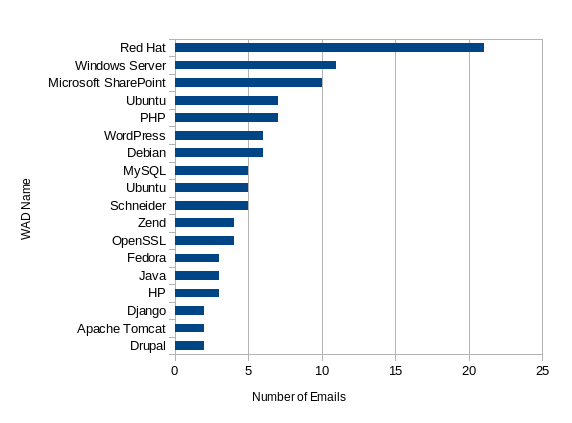
\includegraphics[width=1.0\textwidth]{emails_per_wad}
  \caption{Number of Emails per WAD Name}
\end{figure}


\begin{figure}[h!]
\label{figure:emails_per_wad_fp}
  \centering
    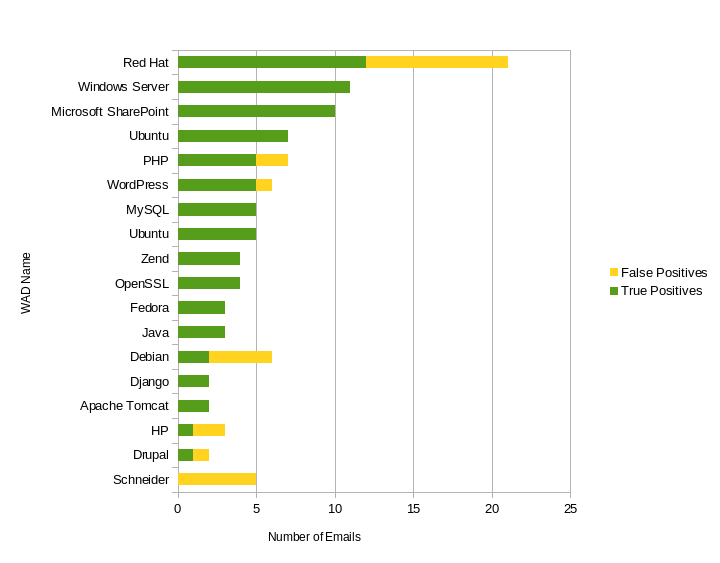
\includegraphics[width=1.0\textwidth]{emails_per_wad_fp}
  \caption{Number of Emails per WAD Name}
\end{figure}


\begin{figure}[h!]
\label{figure:fp_rate}
  \centering
    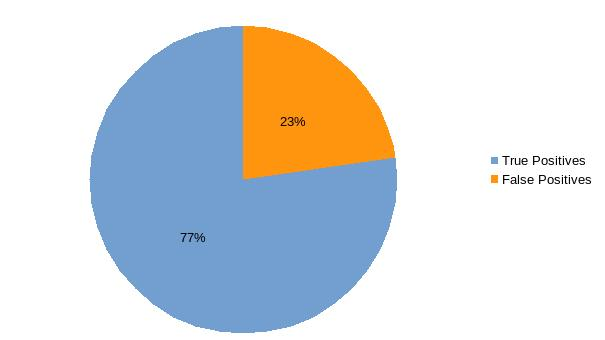
\includegraphics[width=1.0\textwidth]{fp_rate}
  \caption{False Pasitive Rate in Name Matching}
\end{figure}



\begin{figure}[h!]
\label{figure:updates}
  \centering
    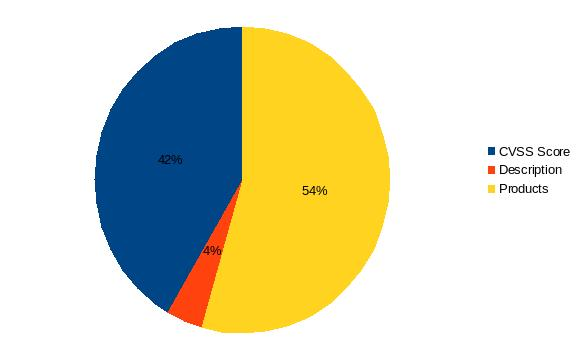
\includegraphics[width=1.0\textwidth]{updates}
  \caption{Updated Fields in Vulnerabilities}
\end{figure}



